\section{Anforderungen}\label{l:anforderungen}

Aus den Ausführungen in der Analyse des Problems in Abschnitt~\ref{l:problemanalyse}~(S.~\pageref{l:problemanalyse}~ff.), der Beschreibung der Personas in Abschnitt~\ref{l:personas}~(S.~\pageref{l:personas}~ff.) und der Konzeption der Anwendung in Abschnitt~\ref{l:konzeption}~(S.~\pageref{l:konzeption}~ff.) sich funktionale und nicht-funktionale Anforderungen an die Anwendung ableiten, die in den Abschnitten \ref{l:funktionale-anforderungen} bzw. \ref{l:nicht-funktionale-anforderungen} beschrieben werden. Die Anforderungen beziehen sich dabei in erster Linie auf die browserbasierte Web-Anwendung und den Webservice. 

\subsection{Funktionale Anforderungen}\label{l:funktionale-anforderungen}

Zur Beschreibung der Anwendung wurde ein vereinfachtes strukturiertes Format nach \cite[S.151~ff.]{schienmann2002kontinuierliches} gewählt, das wie folgt aufgebaut ist: Der \emph{Identifier} einer Anforderung ist die Abschnittsnummer, z.B. \ref{anforderung:registrierung},  die \emph{Kurzbeschreibung} ist der Abschnittstitel. In dem Abschnitt wird die \emph{Zielsetzung} der Anforderung dann beschrieben. Die \emph{Quelle} gibt die Herkunft bzw. den Anforderungssteller an und unter \emph{Domänenobjekte} sind die betroffenen Geschäftsobjekte aufgelistet. Die optionalen \emph{Anmerkungen} listen zusätzliche Bemerkungen und Klarstellungen

\subsubsection{Benutzerkonto}\label{anforderung:registrierung}

Ein Nutzer muss sich mit Hilfe seiner E-Mail-Adresse ein Benutzerkonto im System anlegen können. Hierzu gibt er seine E-Mail-Adresse an. Das System generiert ein Passwort und versendet dieses an die angegebene E-Mail-Adresse. Anschließend kann sich der Benutzer mit diesem Passwort einloggen. Nach dem ersten Login wird er gebeten sein Profil zu vervollständigen. Hat der Nutzer sein Passwort vergessen, kann er im Login-Bereich der Anwendung ein neues Passwort anfordern. Dazu muss er seine E-Mail-Adresse angeben. Wird diese E-Mail-Adresse gefunden, wird ein Passwort-Zurücksetzen-Schlüssel erzeugt und per E-Mail an die Adresse versandt. Ein Link in dieser E-Mail öffnet die Anwendung diesem Schlüssel. Passt der übergebene Schlüssel zum gespeicherten Schlüssel wird ein neues Passwort erzeugt und dem Nutzer per E-Mail zugesendet.

\textsf{Quelle:} Basisanforderung

\textsf{Domänenobjekte:} \texttt{Benutzer \ref{model:benutzer}}

\subsubsection{Definition von Projekten}\label{anforderung:definition-projekt}

Es muss möglich sein, Projekte anzulegen und zu bearbeiten. Projekte bildet den Rahmen für alle Texte eines einzelnen Produktes. Jeder Benutzer kann neue Projekte anlegen. Beim Anlegen eines Projektes wird auch mindestens eine Sprache angelegt, in der die Texte erstellt werden sollen. Es können weitere Sprachen hinzugefügt werden.

\textsf{Quelle:} Basisanforderung

\textsf{Domänenobjekte:} \texttt{Projekt \ref{model:projekt}},  \texttt{Sprache \ref{model:sprache}}

\subsubsection{Definition der Projektstruktur}

Es muss möglich sein, Gruppen anzulegen. Die hierarchische Projektstruktur wird innerhalb eines Projektes mit Hilfe von Gruppen definiert. 

\textsf{Quelle:} Basisanforderung

\textsf{Domänenobjekte:} \texttt{Gruppe \ref{model:gruppe}}

\subsubsection{Definition von Textbausteinen}

Grundlage für die Verwendung eines Textbausteines im Projekt ist dessen Definition. Es muss möglich sein, Textbausteines innerhalb des Projektes zu erzeugt und in dessen Struktur einzuordnet. Dabei muss ein Identifier angegeben werden, der innerhalb des Projektes einmalig ist. Wird kein Identifier angegeben, wird dieser vom System automatisch erzeugt. Zusätzlich ist die Einordnung des Textbausteines innerhalb der Struktur erforderlich. Nach der Definition eines Textbausteines ist dessen Status \texttt{Leer}.

\textsf{Quelle:} Basisanforderung

\textsf{Domänenobjekte:} \texttt{Textbaustein \ref{model:textbaustein}}

\subsubsection{Befüllen von Textbausteinen}

Es muss möglich sein den Inhalt eines Testbausteines anzugeben. Hierzu wird Text zu einem Textbaustein in einer der Projektsprachen eingegeben. Ist bereits ein Inhalt vorhanden, wird eine neue Version angelegt. Nach der Definition eines Textbausteines ist dessen Status \texttt{Befüllt}.

\textsf{Quelle:} Basisanforderung

\textsf{Domänenobjekte:} \texttt{Textbaustein \ref{model:textbaustein}}

\subsubsection{Befüllen von Textbausteinen}

Es muss möglich sein den Inhalt eines Testbausteines anzugeben. Hierzu wird Text zu einem Textbaustein in einer der Projektsprachen eingegeben. Ist bereits ein Inhalt vorhanden, wird eine neue Version angelegt. Nach der Definition eines Textbausteines ist dessen Status \texttt{Befüllt}.

\textsf{Quelle:} Basisanforderung

\textsf{Domänenobjekte:} \texttt{Textbaustein \ref{model:textbaustein}}

\TODO

\subsubsection{Korrigieren von Textbausteinen}

\subsubsection{Prüfen von Textbausteinen}

\subsubsection{Freigeben von Textbausteinen}

\subsubsection{Veröffentlichen von Textbausteinen}

\subsubsection{Gleichzeitiges Bearbeiten von Textbausteinen}

Es soll möglich sein, dass alle  Mitarbeiter gleichzeitig an den Texten eines Produktes arbeiten.

\subsubsection{Festlegung eines Workflows auf Basis des Status}

Abbildung~\ref{chart:statimitworkflow}~(S.~\pageref{chart:statimitworkflow}) zeigt die Abfolge mit Korrekturschleifen. Die Abfolge kann in beide Richtungen erfolgen und auch mehrere Stati überspringen.

\begin{figure}[htb]
\begin{center}
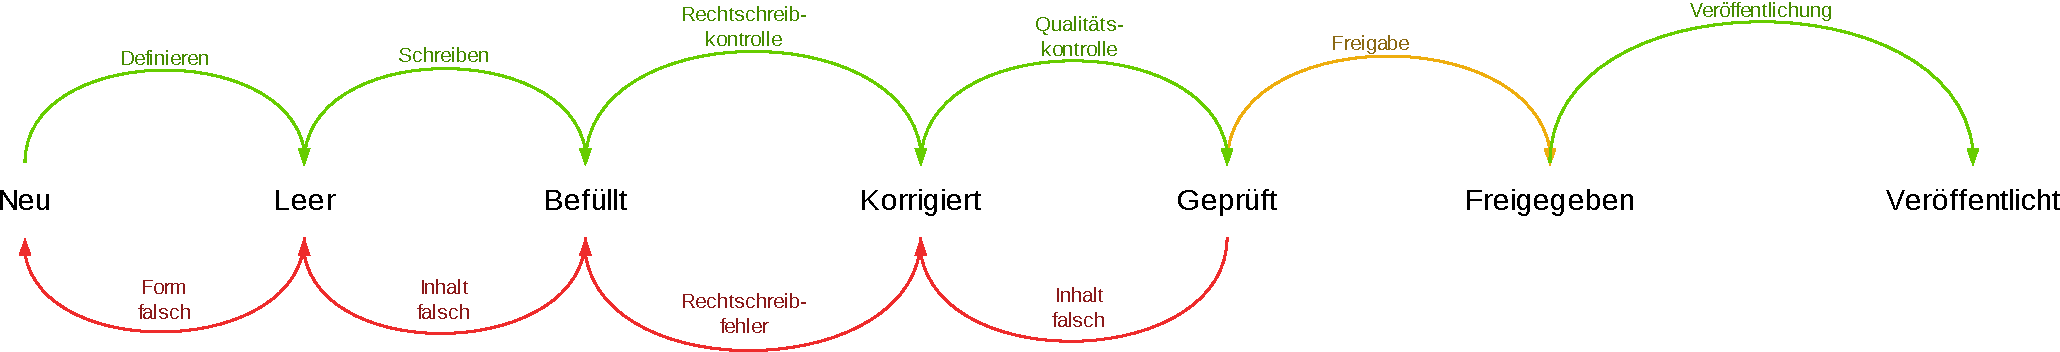
\includegraphics[width=\textwidth]{media/stati-mit-workflow.pdf}
\end{center}
\caption{Ablauf von Statusänderungen}
\label{chart:statimitworkflow}
\end{figure}

\subsubsection{Definieren von Textklassen}

\paragraph{Typ} Überschrift, Untertitel, Bild-Beschreibung, Fließtext.

\subsubsection{Definieren von Textlängebeschränkungen}

\subsubsection{Definieren von Positionen im Produkt}

\subsubsection{Schnittstellen}

\paragraph{Schnittstellen}

Anforderungen, Umfang, Ausprägung für Import-, Export- und Benachrichtigungsschnittstellen

Anbindung via CMIS http://en.wikipedia.org/wiki/Content\_Management\_Interoperability\_Services

\subsection{Nicht-Funktionale Anforderungen}\label{l:nicht-funktionale-anforderungen}

\begin{itemize}
\item Zuverlässigkeit (Systemreife, Wiederherstellbarkeit, Fehlertoleranz)
\item Aussehen und Handhabung (Look and Feel)
\item Benutzbarkeit (Verständlichkeit, Erlernbarkeit, Bedienbarkeit)
\item Leistung und Effizienz (Antwortzeiten, Ressourcenbedarf, Wirtschaftlichkeit)
\item Betrieb und Umgebungsbedingungen
\item Wartbarkeit, Änderbarkeit (Analysierbarkeit, Stabilität, Prüfbarkeit, Erweiterbarkeit)
\item Portierbarkeit und Übertragbarkeit (Anpassbarkeit, Installierbarkeit, Konformität, Austauschbarkeit)
\item Sicherheitsanforderungen (Vertraulichkeit, Informationssicherheit, Datenintegrität, Verfügbarkeit)
\item Korrektheit (Ergebnisse fehlerfrei)
\item Flexibilität (Unterstützung von Standards)
\item Skalierbarkeit (Änderungen des Problemumfangs bewältigen)
\item Randbedingungen
\end{itemize}
